\documentclass{article}

\usepackage{fancyhdr}
\usepackage{extramarks}
\usepackage{amsmath}
\usepackage{amsthm}
\usepackage{amsfonts}
\usepackage{tikz}
\usepackage[plain]{algorithm}
\usepackage{algpseudocode}
\usepackage[encapsulated]{CJK}
\usepackage{graphicx}
\usepackage{caption}
\usepackage{subcaption}
\graphicspath{ {./images/} }

\usetikzlibrary{automata,positioning}

%
% Basic Document Settings
%

\topmargin=-0.45in
\evensidemargin=0in
\oddsidemargin=0in
\textwidth=6.5in
\textheight=9.0in
\headsep=0.25in

\linespread{1.1}

\pagestyle{fancy}
\lhead{\hmwkAuthorName}
\chead{\hmwkClass\:\hmwkTitle}
\rhead{\firstxmark}
\lfoot{\lastxmark}
\cfoot{\thepage}

\renewcommand\headrulewidth{0.4pt}
\renewcommand\footrulewidth{0.4pt}

\setlength\parindent{0pt}

%
% Create Problem Sections
%

\newcommand{\enterProblemHeader}[1]{
    \nobreak\extramarks{}{Problem \arabic{#1} continued on next page\ldots}\nobreak{}
    \nobreak\extramarks{Problem \arabic{#1} (continued)}{Problem \arabic{#1} continued on next page\ldots}\nobreak{}
}

\newcommand{\exitProblemHeader}[1]{
    \nobreak\extramarks{Problem \arabic{#1} (continued)}{Problem \arabic{#1} continued on next page\ldots}\nobreak{}
    \stepcounter{#1}
    \nobreak\extramarks{Problem \arabic{#1}}{}\nobreak{}
}

\setcounter{secnumdepth}{0}
\newcounter{partCounter}
\newcounter{homeworkProblemCounter}
\setcounter{homeworkProblemCounter}{1}
\nobreak\extramarks{Problem \arabic{homeworkProblemCounter}}{}\nobreak{}

%
% Homework Problem Environment
%
% This environment takes an optional argument. When given, it will adjust the
% problem counter. This is useful for when the problems given for your
% assignment aren't sequential. See the last 3 problems of this template for an
% example.
%
\newenvironment{homeworkProblem}[1][-1]{
    \ifnum#1>0
        \setcounter{homeworkProblemCounter}{#1}
    \fi
    \section{Problem \arabic{homeworkProblemCounter}}
    \setcounter{partCounter}{1}
    \enterProblemHeader{homeworkProblemCounter}
}{
    \exitProblemHeader{homeworkProblemCounter}
}

%
% Homework Details
%   - Title
%   - Due date
%   - Class
%   - Section/Time
%   - Instructor
%   - Author
%

\newcommand{\hmwkTitle}{Homework\ \#2}
%\newcommand{\hmwkDueDate}{September 17, 2015}
\newcommand{\hmwkClass}{Graph Theory}
\newcommand{\hmwkClassTime}{}
\newcommand{\hmwkClassInstructor}{}
\newcommand{\hmwkAuthorName}{Lin Hung Cheng B01902059}

%
% Title Page
%

\title{
    \vspace{2in}
    \textmd{\textbf{\hmwkClass:\ \hmwkTitle}}\\
    %\normalsize\vspace{0.1in}\small{Due\ on\ \hmwkDueDate\ at 3:10pm}\\
    %\vspace{0.1in}\large{\textit{\hmwkClassInstructor\ \hmwkClassTime}}
    \vspace{3in}
}

\author{\textbf{\hmwkAuthorName}}
\date{}

\renewcommand{\part}[1]{\textbf{\large Part \Alph{partCounter}}\stepcounter{partCounter}\\}

%
% Various Helper Commands
%

% Useful for algorithms
\newcommand{\alg}[1]{\textsc{\bfseries \footnotesize #1}}

% For derivatives
\newcommand{\deriv}[1]{\frac{\mathrm{d}}{\mathrm{d}x} (#1)}

% For partial derivatives
\newcommand{\pderiv}[2]{\frac{\partial}{\partial #1} (#2)}

% Integral dx
\newcommand{\dx}{\mathrm{d}x}

% Alias for the Solution section header
\newcommand{\solution}{\textbf{\large Solution}}

% Probability commands: Expectation, Variance, Covariance, Bias
\newcommand{\E}{\mathrm{E}}
\newcommand{\Var}{\mathrm{Var}}
\newcommand{\Cov}{\mathrm{Cov}}
\newcommand{\Bias}{\mathrm{Bias}}

\begin{document}

\maketitle

\pagebreak

\begin{homeworkProblem}
  \begin{CJK}{UTF8}{bsmi} % 開始 CJK
    試證明, 每一個連通近圖都有一條道路, 將此近圖中的一條邊至少用過一次。甚至可以進一步要求,任一條邊都用了一次或兩次。

    \proof
    至少用過一次:對一圖G,從點$V \in G$開始,分別走向所有$V_n \in Neighbor(V)$,再走回V,其路徑為$VV_1VV_2VV_3....V_n$,完成後,因為是連通圖,可走到任意一個尚未執行此步驟的點W,分別走向所有$W_n \in Neighbor(W)$,再走回W......重複執行直到所有在G中的點都執行過此步驟。\\
    此時G中的所有點都走過其所有的邊,所以任一條邊至少用過一次。\\

    因為此種走法有許多不必要的重複,若一條邊被行走超過兩次,可以將在行走路徑中最近的 $(a \rightarrow b), (b \rightarrow a)$成對刪除,最後每一條邊會剩下1次或2次行走。\\
    因為在 $(a\rightarrow b), (b \rightarrow a)$ 之間的路徑序列則可能是 從a到a,或是 從b到b 的路徑,可以將此序列移動到剩下的 $(X \rightarrow a), (X \rightarrow b)$後面,或$(a \rightarrow X) , (b \rightarrow X)$前面,而不會影響其他行走序列。
  \end{CJK}
\end{homeworkProblem}

\begin{homeworkProblem}
  \begin{CJK}{UTF8}{bsmi} % 開始 CJK
    試證明, 對$1 \leq k \leq 8$ 有向近圖$G_{2,4}$ 都有一條長度為k 的有向圈。是否對$1 \leq k \leq σ^{n-1}$ 有向近圖$G_{σ^{n-1}}$ 都有一條長度為k 有向圈?\\

    \textbf{Solution}

    k = 1,111-111\\
    k = 2,101-010-101\\
    k = 3,101-011-110-101\\
    k = 4,111-110-101-011-111\\
    k = 5,111-110-100-001-011-111\\
    k = 6,111-110-101-010-101-011-111\\
    k = 7,111-110-100-001-010-101-011-111\\
    k = 8,111-110-100-000-001-010-101-011-111\\
    有向近圖$G_{σ^{n-1}}$若要有 長度為k的cycle
    設起始點為V = {a0, a1, a2 ...},其cycle路徑為\\
    $\{a_1a_2a_3...a_n,  a_2a_3...a_nb_1,  a_3...a_nb_1b_2,  ... , b_1...b_k\}$\\
    必有k = 1的cycle,如111...1 - 111...1
    若沒有 k = n的cycle,則
    
  \end{CJK} % 結束 CJK 環境 
\end{homeworkProblem}

\pagebreak

\begin{homeworkProblem}
  \begin{CJK}{UTF8}{bsmi} % 開始 CJK
    下面的序列何者為圖序列?若是,請構造出對應的圖;若不是,請說明理由。\\
    (5, 5, 4, 3, 2, 2, 2, 1), (5, 5, 5, 3, 2, 2, 1, 1), (5, 5, 4, 4, 2, 2, 1, 1), (5, 5, 5, 4, 2, 1, 1, 1)。\\

    \solution
    \\
    用定理1.17 確定是否是圖序列\\
    \textbf{1.}
    $(5, 5, 4, 3, 2, 2, 2, 1) \rightarrow (4, 3, 2, 2, 1, 1, 1) \rightarrow (2, 1, 1, 1, 1, 0) \rightarrow (1, 1)\rightarrow (0)$\\
    $d_1 = 0$,滿足是圖序列的條件\\
    \textbf{2.}
    $(5, 5, 5, 3, 2, 2, 1, 1) \rightarrow (4, 4, 2, 1, 1, 1, 1) \rightarrow (3, 1, 1, 1) \rightarrow (0) $\\
    $d_1 = 0$,滿足是圖序列的條件\\
    \textbf{3.}
    $(5, 5, 4, 4, 2, 2, 1, 1) \rightarrow (4, 3, 3, 1, 1, 1, 1) \rightarrow (2, 2, 1, 1) \rightarrow (1, 1, 0) \rightarrow (0)$\\
    $d_1 = 0$,滿足是圖序列的條件\\
    \textbf{4.}
    $(5, 5, 5, 4, 2, 1, 1, 1) \rightarrow (4, 4, 3, 1, 1, 1) \rightarrow (3, 2, 1)$\\
    $d_1 > 2$,不滿足圖序列的條件

    \begin{figure}[h]
      \centering
      \begin{subfigure}[b]{0.3\textwidth}
        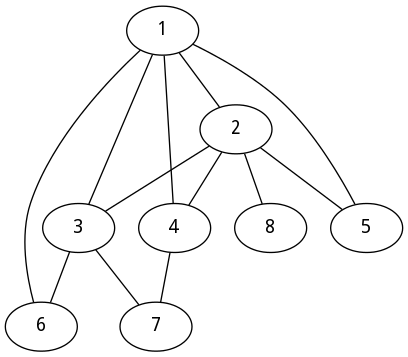
\includegraphics[width=\textwidth]{graph1.png}
        \centering
        1
      \end{subfigure}
      ~ %add desired spacing between images, e. g. ~, \quad, \qquad, \hfill etc. 
      % (or a blank line to force the subfigure onto a new line)
      \begin{subfigure}[b]{0.3\textwidth}
        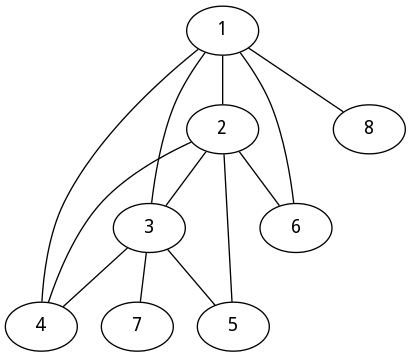
\includegraphics[width=\textwidth]{graph2.png}
        \centering
        2
      \end{subfigure}
      ~ %add desired spacing between images, e. g. ~, \quad, \qquad, \hfill etc. 
      % (or a blank line to force the subfigure onto a new line)
      \begin{subfigure}[b]{0.3\textwidth}
        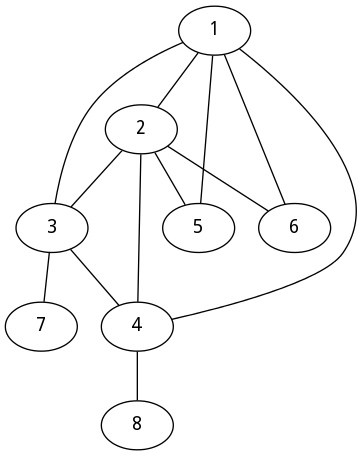
\includegraphics[width=\textwidth]{graph3.png}
        \centering
        3
      \end{subfigure}
      \centering
      Answer
    \end{figure}    
  \end{CJK} % 結束 CJK 環境 
\end{homeworkProblem}

\begin{homeworkProblem}
  \begin{CJK}{UTF8}{bsmi} % 開始 CJK
    對兩個排序的非負整數序列a: $a_1 \geq a_2 \geq ... \geq a_m$ 和b : $b_1 \geq b_2 \geq ... \geq b_n$,試證明,存在一個二分圖其兩部分的度序列分別是a 和b 的充分必要條件。\\
    \solution

    已知 $a_1^* \geq a_2^* \geq ... \geq a_k^*$,\\
    且屬於$a_k^*$的點$\in$屬於$a_{k-1}^*$的點$\in ... \in$ 屬於$a_1^*$的點\\
    
    \textbf{1.}
    存在二分圖 $\Rightarrow$ $\sum_{i=1}^{m}{a_i} = \sum_{j=1}^{n}{b_j}$ 且 $a_1^* + a^*_2 + ... + a_k^* \geq b_1 + b_2 + b_3 + ... + b_k$\\
    因為二分圖的邊只存在於a部份和b部份的連線,兩邊度數和會相同。\\
    k = 1時,$a_1^* \geq b_1$ 明顯成立,否則$b_1$代表的點無法連到$b_1$個不同的點。\\
    k = 2時,$b_2$和$b_1$可以都連到屬於$a_2^*$的點,此時a部份剩下$a_1^*-a_2^*$個點可供$b_1$或$b_2$其中一個連,所以$b_2+b_1 \leq (a_1^*-a_2^*)+a_2^* \times 2 = a_1^* + a_2^*$\\
    以此方法類推,則$a_1^* + a^*_2 + ... + a_k^* \geq b_1 + b_2 + b_3 + ... + b_k$成立,右式得證
    
    \textbf{2.}
    存在二分圖 $\Leftarrow$ $\sum_{i=1}^{m}{a_i} = \sum_{j=1}^{n}{b_j}$ 且 $a_1^* + a^*_2 + ... + a_k^* \geq b_1 + b_2 + b_3 + ... + b_k$\\
    從子圖$G = (V(G),\emptyset)$, 將$b_1$代表的點連到$b_1$個符合$a_1^*$的點,而且從屬於$a_k^*$的點開始連,再連到屬於$a_{k-1}^*$的點...以此類推。因為$a_1^* \geq b_1$,必有成功的連接。\\
    將$b_2$代表的點連到$b_2$個符合$a_2^*$的點,因為$a_1^* + a_2^* \geq b_1 + b_2$且$a_1^* \geq b_1$,所以$a_2^* \geq b_2$,必有成功的連接。因為$\sum_{i=1}^{m}{a_i} = \sum_{j=1}^{n}{b_j}$,以此方式對$b_1 ... b_j$作連線後,a部份的點也會全部連線,可得所述的二分圖\\

    % 由上述兩式相減,可得$a_2^* \geq b_2$,依數學歸納法可知 $a_n^* \geq b_n$ \\
    %a_1^* + a^*_2 + ... + a_j^* \geq b_1 + b_2 + b_3 + ... + b_j$明顯成立(等號),\\
    %$a_1^* + a^*_2 + ... + a_{j-1}^* \geq b_1 + b_2 + b_3 + ... + b_{j-1}$明顯成立(等號),\\
  \end{CJK} % 結束 CJK 環境 
\end{homeworkProblem}

\begin{homeworkProblem}
  \begin{CJK}{UTF8}{bsmi} % 開始 CJK
    一個山脈是指坐標平面上從A = (a, 0) 到B = (b, 0) 在上半平面的一連串折線段。考慮兩個登山者A 和B 分別從兩端點出發, 試證明,他們有辦法用一種(或許是非常詭異的)方式登山、使得兩個人在登山過程中的任何時刻都維持在同樣的海拔高度,而且最後又能碰面。(提示:請試著用一個圖來模擬兩個登山者的移動)

    \solution

    將山峰和山谷(圖中的極大值和極小值)視為節點\\
    當A或B遇到節點的時候,若要繼續前進,則另一個人需要改變方向才能維持高度相同。\\
    所以走法為:當A或B遇到節點的時候,繼續前進,另一個人改變方向,若同時遇到節點則不需要改變方向。\\
    %當A或B在前進到下一個節點V的過程,另一人最終將會退到和V高度相同的位置W,而這個過程是有限次的。\\
    設A改變方向,B的目前高度為$h_1$,下一個將到的節點高度為$h_2$,則在B到達$h_2$之前,A的高度只會在$h_1$和$h_2$之間移動,也就是說,B不會退到目前的節點之前,這可以保證B可以在A遇到有限次節點後,走到下一個節點。而整個圖包含有限個節點,所以B可以在遇到有限次節點的情況下遇到A。\\
    \proof
    若改變方向後,A到達$h_2$高度前,遇到的節點高度為h,在不失一般性的情況下,設$h_1>h_2$:
    \begin{enumerate}
    \item 若$h < h_2$,B會先到達下一個節點,符合條件
    \item 若$h_1 > h > h_2$,符合條件
    \item 若$h > h_1$, 則在此節點前,至少有一節點在$h_1, h_2$之間(因為從變低到變高)令A改變方向後第一個遇到的節點為C,因為C比B在$h_1$的節點早遇到,在遇到C的時候,A會前進,且B會改變方向,所以B不會先達到$h_1$,而是A先達到下一個節點,矛盾
    \end{enumerate}
\end{CJK} % 結束 CJK 環境 
\end{homeworkProblem}

\end{document}

%%% Local Variables:
%%% mode: latex
%%% TeX-master: t
%%% End:
